\section{Baseline Model}
This model is inspired by the CNN+MLP model used by \textcite{Santoro} on their Sort-of-CLEVR dataset and modified in resemblance to the VGG-16 architecture introduced by \textcite{Simonyan2014}. The overall architecture of this model includes a convolutional neural network (CNN) which extracts features from the input image, followed by a fully connected network (also referred to as a multilayer perceptron, or MLP) which processes the extracted features and query into an answer (\textit{`Is there a red object?' $\to$  `yes'}). 

A convolutional neural network (CNN) is a neural network architecture often used in computer vision problems, or other domains where the input has a spatial structure where we expect some degree of spatial invariance -- in our task, a sphere should be recognized as a sphere regardless of where in the image it appears. Each layer group in our CNN begins with the convolutional layer, which applies a set of filters at every location in the image (the convolution operation). After each filter computes a value at every location, the layer group continues with a nonlinearity function, batch normalization (in order to account for differences between batches), and local pooling (in order to reduce the spatial dimensions between layer groups). The specific architecture employed in this model includes four layer groups, with 16, 32, 48, and 64 filters in each one. Each filter is 3x3 units, moved with a stride of 1 and padding of 1, and the pooling units reduce each 2x2 unit block to a single unit - halving the input size between layers, or doubling the effective receptive field of units between layers. The output of the last convolutional layer group has dimensions 64 (filters) x 10 (width) x 7 (height). 

To feed the convolutional output to the next, fully connected layer, we need to flatten it, as fully connected layers receive a vector as their input. We, therefore, flatten the output above to a $64 \times 10 \times 7 = 4480$ unit vector, to which we concatenate the 30-unit query representation, arriving at a 4510-unit input to the fully connected network. The fully connected network has four such layers, each with 512 hidden units, also using the ReLU activation function, before the final layer, which has two units. We interpret these units as the probability assigned to `yes' and the probability assigned to `no’ on our binary queries. We used the cross-entropy loss function, which evaluates the model based on how much of the probability mass the model assigned to the correct answer. 

The following schematic describes the model: the initial blocks are the convolutional ones, where the layers retaining spatial size and increase depth are the convolutions, and the layers maintaining depth and reducing size are the pooling ones. The eventual representation is flattened, the query is appended to it, and it is then passed to the fully connected layers.
\begin{figure}[!htb]
% \vspace{-0.225in}
\centering
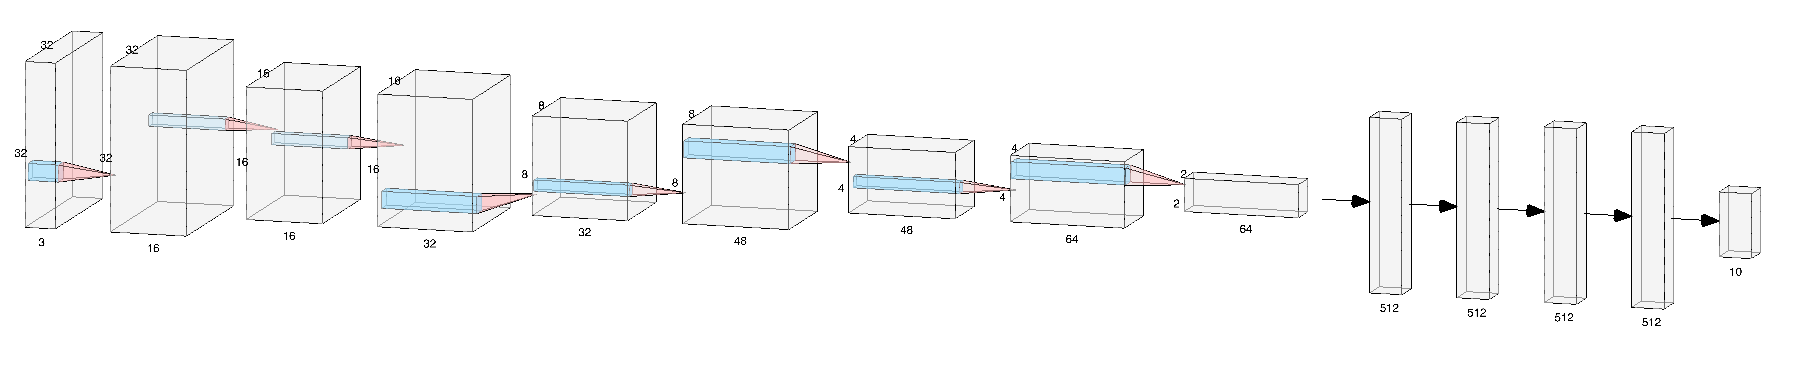
\includegraphics[width=\linewidth]{ch-models-compared/figures/baseline.png}
\caption{{\bf Baseline model diagram.} The schematic does not include the concatenated query, and has ten output units, whereas in this case there are two units, yes and no. }
\label{fig:baseline-model-diagram}
% \vspace{-0.2in}
\end{figure}

Initial experiments on the entire dataset, presenting all thirty single-feature tasks together, demonstrated that the model was overfitting the training set, as at some point through training, the test-set accuracy and loss stagnated, while the loss on the training set continued dropping, and correspondingly, the training set accuracy continued rising. We then experimented with several measures designed to prevent overfitting. Dropout is one such measure, which during training randomly turns off random units in each layer, intuitively forcing the network to learn to build in some redundancy to how it solves the task, therefore improving its robustness. We experimented with both forms of dropout, standard \parencite{Srivastava2014} for the fully-connected layer, and spatial dropout \parencite{Tompson2015}, which turns off entire filters (again, encouraging redundancy between them) in convolutional part of the network. Another measure we attempted is weight decay \parencite{Krogh1992}, which puts a small penalty on the magnitude of the weights, encouraging weights to remain smaller (and corresponding to a zero-mean Gaussian prior on the weights). We also introduced a learning rate scheduler, to reduce the learning rate when the network gets “stuck,” allowing it to perform granular tuning at that point. Of these, weight decay proved by far the most effective (see results below), the learning rate scheduler only helped with minor tuning, and dropout proved ineffective. Therefore, we perform the sequential benchmark experiments reported below with weight decay (using a penalty of 1e-4) and without the learning rate scheduler or dropout. All models were fit using the Adam \parencite{Kingma2015} optimizer.